\subsection{Backpropagation for a simple network}


Da man mit zufälligen Anfangsgewichten arbeitet kann es vorkommen das man auch lokale Minima findet.
Dies ist sehr stark von den Werten der Anfangsgewichte abhängig. Bei ``schlechten Startgewichten'' kann es vorkommen das man in ein Lokales Minima läuft und dort ``hängen'' bleibt.

\subsubsection{Formeln für Forwardfeed}

Zuerst werden die Eingänge entsprechend der W(1)-Matrix gewichtet und aufsummiert.
\begin{equation}
\vect{a}^{(1)} = [\vect{x},1] * \vect{W}^{(1)}
\end{equation}

Die Summe der gewichteten Eingänge wird anschließend durch die Aktivierungsfunktion $\sigma(x)$ geschickt.

\begin{equation}
\vect{z} = \sigma(\vect{a}^{(1)})
\end{equation}

Anschließend wird werden die Ausgänge der Neuronen (z) mit der W(2)-Matrix gewichtet und aufsummiert:

\begin{equation}
 \vect{a}^{(2)} = [z,1] * \vect{W}^{(2)}
\end{equation}

Die Summe der gewichteten Neuronenausgänge im Hidden Layer wird anschließend wieder durch die Aktivierungsfunktion $\sigma(x)$ geschickt.
\begin{equation}
 output = \sigma(\vect{a}^{(2)})
\end{equation}



\subsubsection{Formulen für Backpropagation}

Gewichtsänderung für den Output Layer:
\begin{equation}
 \frac{\partial E}{\partial w_{kj}^{(2)}} = \frac{\partial E}{\partial a_{k}^{(2)}} \frac{\partial a_{k}^{(2)}}{\partial w_{kj}^{(2)}} = \delta_k^{(2)} z_j
\end{equation}

Gewichtsänderung für den Hidden Layer:
\begin{equation}
 \frac{\partial E}{\partial w_{ji}^{(1)}} = \frac{\partial E}{\partial a_{j}^{(1)}} \frac{\partial a_{j}^{(1)}}{\partial w_{ji}^{(1)}} = \delta_j^{(1)} x_i
\end{equation}

Fehler berechung $\delta^{(j)}$ für Output Layer:
\begin{equation}
 \delta_k^{(2)} = h_{(2)}' (a_k^{(2)}) 2 (o_k - y_k)
\end{equation}
Fehler berechung $\delta^{(j)}$ für Hidden Layer:

\begin{equation}
 \delta_j^{(1)} = h_{(1)}' (a_j^{(1)}) \sum\limits_{k=1}^n w_{kj}^{(2)} \delta_k^{(2)}
\end{equation}



\begin{figure}[hp!]
\begin{center}
 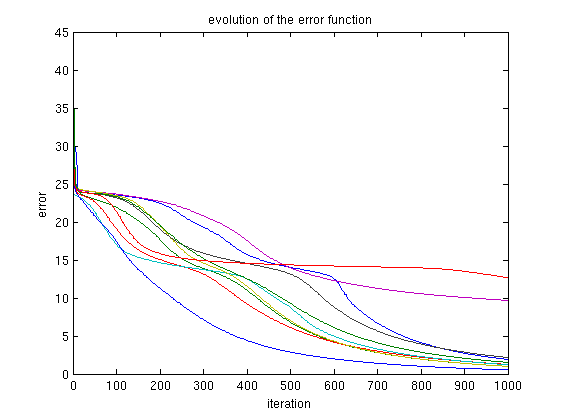
\includegraphics[width=0.99\textwidth]{./figures/1/error}
 \caption{Evolution of the error over the iterations with different startweight-vectors}
\label{fig:backprop_error}
\end{center}
\end{figure}



\begin{figure}[hp!]
\begin{center}
 \begin{minipage}{0.48\textwidth}
 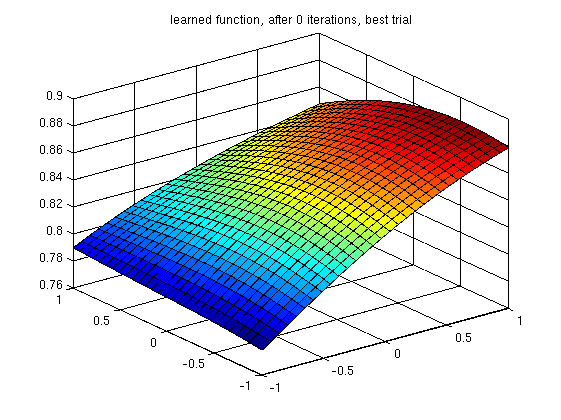
\includegraphics[width=0.99\textwidth]{./figures/1/learned_best_0}
 \end{minipage}
 \begin{minipage}{0.48\textwidth}
 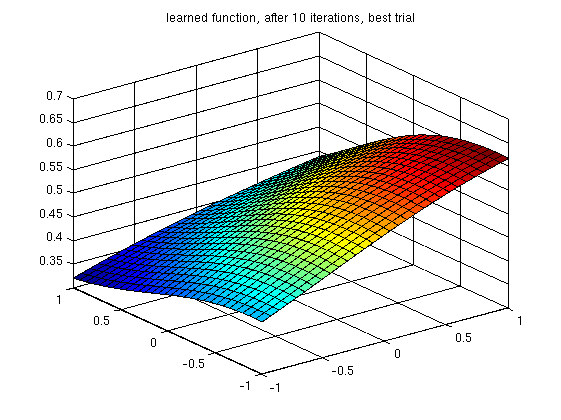
\includegraphics[width=0.99\textwidth]{./figures/1/learned_best_10}
 \end{minipage}
 \begin{minipage}{0.48\textwidth}
 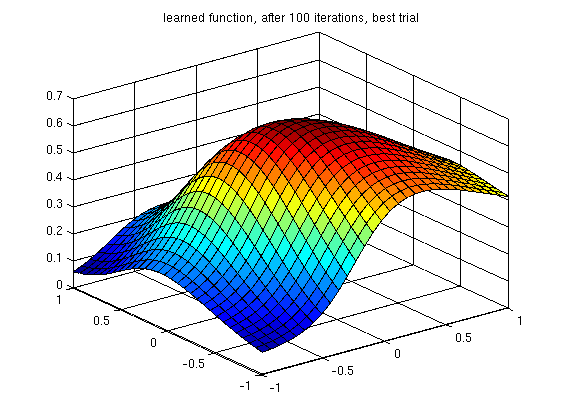
\includegraphics[width=0.99\textwidth]{./figures/1/learned_best_100}
 \end{minipage}
 \begin{minipage}{0.48\textwidth}
 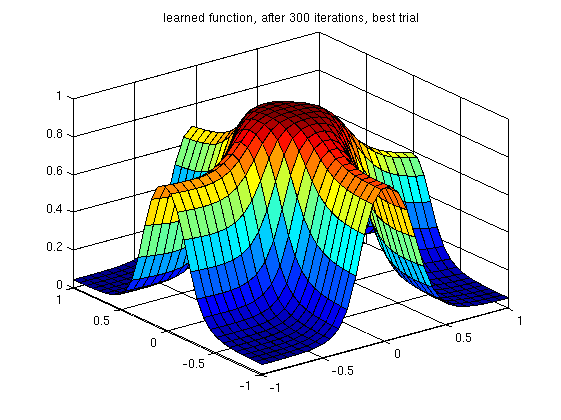
\includegraphics[width=0.99\textwidth]{./figures/1/learned_best_300}
 \end{minipage}
 \begin{minipage}{0.48\textwidth}
 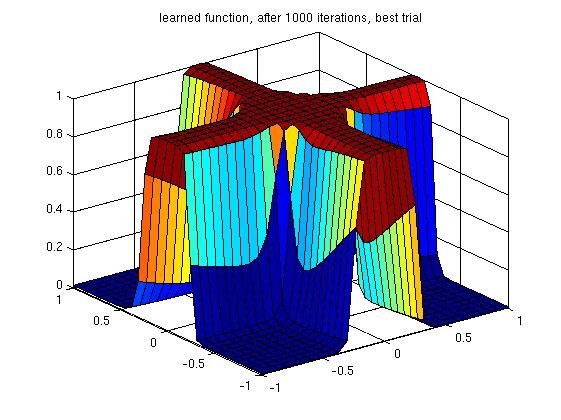
\includegraphics[width=0.99\textwidth]{./figures/1/learned_best_1000}
 \end{minipage}
 \caption{Learned Function after 0,10,100,300,1000 Iterations(Best Trial)}
\label{fig:learned_function_best}
\end{center}
\end{figure}


\begin{figure}[hp!]
\begin{center}
 \begin{minipage}{0.48\textwidth}
 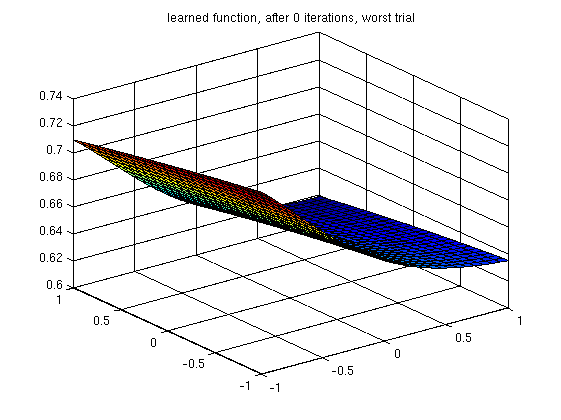
\includegraphics[width=0.99\textwidth]{./figures/1/learned_worst_0}
 \end{minipage}
 \begin{minipage}{0.48\textwidth}
 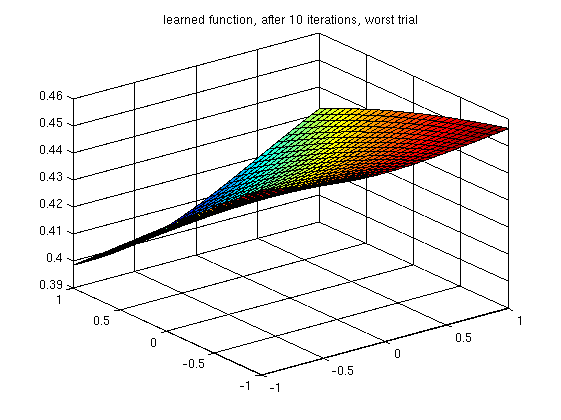
\includegraphics[width=0.99\textwidth]{./figures/1/learned_worst_10}
 \end{minipage}
 \begin{minipage}{0.48\textwidth}
 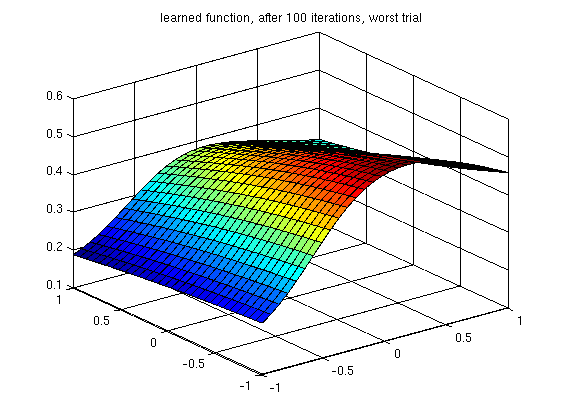
\includegraphics[width=0.99\textwidth]{./figures/1/learned_worst_100}
 \end{minipage}
 \begin{minipage}{0.48\textwidth}
 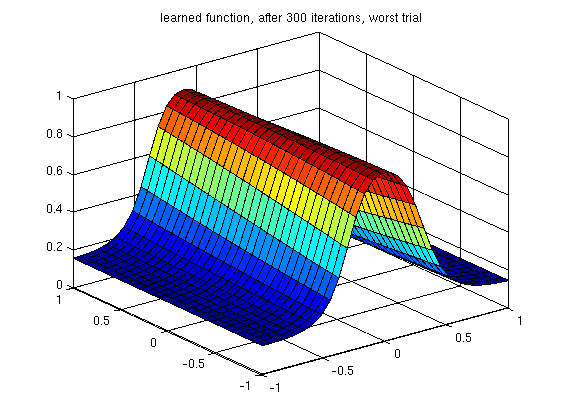
\includegraphics[width=0.99\textwidth]{./figures/1/learned_worst_300}
 \end{minipage}
 \begin{minipage}{0.48\textwidth}
 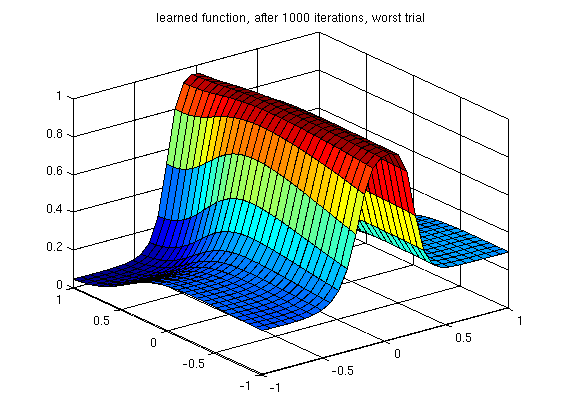
\includegraphics[width=0.99\textwidth]{./figures/1/learned_worst_1000}
 \end{minipage}
 \caption{Learned Function after 0,10,100,300,1000 Iterations(Worst Trial)}
\label{fig:learned_function_worst}
\end{center}
\end{figure}

